%Este trabalho está licenciado sob a Licença Creative Commons Atribuição-CompartilhaIgual 3.0 Não Adaptada. Para ver uma cópia desta licença, visite http://creativecommons.org/licenses/by-sa/3.0/ ou envie uma carta para Creative Commons, PO Box 1866, Mountain View, CA 94042, USA.

%\documentclass[main.tex]{subfiles}
%\begin{document}

\chapter{Solução de sistemas de equações não lineares}\index{sistema de equações!não lineares}
Neste capítulo, estudaremos o método de Newton aplicado à resolução de sistemas não lineares de equações.

O método de Newton aplicado a encontrar a raiz $x^*$ da função $y=f(x)$ estudado na Seção~\ref{metodo_newton_1d} consiste em um processo iterativo. Em cada passo deste processo, dispomos de uma aproximação $x^{(k)}$ para $x^*$ e construímos uma nova aproximação $x^{(k+1)}$.  Cada passo do método de Newton envolve os seguintes procedimentos:
\begin{itemize}
\item Linearização da função $f(x)$ no ponto $x^{(k)}$:
  \begin{equation*}
    f(x)= f(x^{(k)})+ (x-x^{(k)}) f'(x^{(k)}) + O\left(|x-x^{(k)}|^2\right)
  \end{equation*}
\item A aproximação $x^{(k+1)}$ é definida como o valor de $x$ em que a linearização $f(x^{(k)})+ (x-x^{(k)}) f'(x^{(k)})$ passa por zero.
\end{itemize}

%{\bf Observação:} $y=f(x^{(k)})+ (x-x^{(k)}) f'(x^{(k)})$ é a equação da reta que tangencia a curva $y=f(x)$ no ponto $(x^{(k)},f(x^{(k)}))$.

Queremos, agora, generalizar o método de Newton a fim de resolver problemas de várias equações e várias incógnitas, ou seja, encontrar $x_1,x_2,\ldots x_n$ que satisfazem as seguintes equações:

\begin{eqnarray*}
f_1(x_1,x_2,\ldots,x_n)&=&0\\
f_2(x_1,x_2,\ldots,x_n)&=&0\\
&\vdots&\\
f_n(x_1,x_2,\ldots,x_n)&=&0
\end{eqnarray*}

Podemos escrever este problema na forma vetorial definindo o vetor $x=[x_1,x_2,\ldots,x_n]^T$ e a função vetorial
$$F(x)=\left[
\begin{array}{c}
f_1(x_1,x_2,\ldots,x_n)\\
f_2(x_1,x_2,\ldots,x_n)\\
\vdots\\
f_n(x_1,x_2,\ldots,x_n)
\end{array}
\right].$$

\begin{ex} Suponha que queiramos resolver numericamente o seguinte sistema de duas equações e duas incógnitas:
\begin{eqnarray*}
\frac{x_1^2}{3}+x_2^2&=&1\\
x_1^2+\frac{x_2^2}{4}&=&1
\end{eqnarray*}
Então definimos

$$F(x)=\left[
\begin{array}{c}
\frac{x_1^2}{3}+x_2^2-1\\~\\
x_1^2+\frac{x_2^2}{4}-1
\end{array}
\right]$$
\end{ex}
Neste momento, dispomos de um problema na forma $F(x)=0$ e precisamos desenvolver uma técnica para linearizar a função $F(x)$. Para tal, precisamos de alguns conceitos do cálculo de várias variáveis.

Observe que $F(x)-F(x^{(0)})$ pode ser escrito como

$$F(x)-F(x^{(0)})=\left[
\begin{array}{c}
f_1(x_1,x_2,\ldots,x_n)-f_1(x_1^{(0)},x_2^{(0)},\ldots,x_n^{(0)})\\
f_2(x_1,x_2,\ldots,x_n)-f_2(x_1^{(0)},x_2^{(0)},\ldots,x_n^{(0)})\\
\vdots\\
f_n(x_1,x_2,\ldots,x_n)-f_n(x_1^{(0)},x_2^{(0)},\ldots,x_n^{(0)})
\end{array}
\right]$$

Usamos a regra da cadeia
$$df_i = \frac{\partial f_i}{\partial x_1} dx_1+\frac{\partial f_i}{\partial x_2} dx_2+\cdots + \frac{\partial f_i}{\partial x_n} dx_n=\sum_{j=1}^n\frac{\partial f_i}{\partial x_j} dx_j$$
e aproximamos as diferenças por derivadas parciais:
$$ f_i(x_1,x_2,\ldots,x_n)-f_i(x_1^{(0)},x_2^{(0)},\ldots,x_n^{(0)})\approx \sum_{j=1}^n \frac{\partial f_i}{\partial x_j}\left(x_j-x_j^{(0)}\right)$$
Portanto,
\begin{equation}\label{eq_approx_newton}F(x)-F(x^{(0)})\approx \left[
\begin{array}{ccccc}
\frac{\partial f_1}{\partial x_1}&\frac{\partial f_1}{\partial x_2}&\cdots&\frac{\partial f_1}{\partial x_n}\\~\\
\frac{\partial f_2}{\partial x_1}&\frac{\partial f_2}{\partial x_2}&\cdots&\frac{\partial f_2}{\partial x_n}\\~\\
\vdots&\vdots&\ddots&\vdots\\~\\
\frac{\partial f_n}{\partial x_1}&\frac{\partial f_n}{\partial x_2}&\cdots&\frac{\partial f_n}{\partial x_n}\\~\\
\end{array}
\right]\left[
\begin{array}{c}
x_1-x_1^{(0)}\\~~\\
x_2-x_2^{(0)}\\~~\\
\vdots\\~~\\
x_n-x_n^{(0)}
\end{array}
\right],
\end{equation}

Definimos, então, a matriz jacobiana por\index{matrix!jacobiana}
$$J_F= \frac{\partial(f_1,f_2,\ldots,f_n)}{\partial(x_1,x_2,\ldots,x_n)}=\left[
\begin{array}{ccccc}
\frac{\partial f_1}{\partial x_1}&\frac{\partial f_1}{\partial x_2}&\cdots&\frac{\partial f_1}{\partial x_n}\\~\\
\frac{\partial f_2}{\partial x_1}&\frac{\partial f_2}{\partial x_2}&\cdots&\frac{\partial f_2}{\partial x_n}\\~\\
\vdots&\vdots&\ddots&\vdots\\~\\
\frac{\partial f_n}{\partial x_1}&\frac{\partial f_n}{\partial x_2}&\cdots&\frac{\partial f_n}{\partial x_n}\\~\\
\end{array}
\right].
$$
Isto é, a matriz jacobiana de uma função ou simplesmente, o jacobiano de uma função $F(x)$ é a matriz formada pelas suas derivadas parciais:
$$\left(J_F\right)_{ij}=\frac{\partial f_i}{\partial x_j}.$$

Nestes termos, podemos reescrever \eqref{eq_approx_newton} como
$$F(x)\approx F(x^{(0)}) + J_F(x^{(0)}) (x-x^{(0)})$$
Esta expressão é chamada de linearização de $F(x)$ no ponto $x^{(0)}$ e generaliza a linearização em uma dimensão dada por $f(x)\approx f(x^{(0)})+f'(x^{(0)}) (x-x^{(0)})$.

%%%%%%%%%%%%%%%%%%%%
% python
%%%%%%%%%%%%%%%%%%%%
\ifispython
Ao longo deste capítulo, assumiremos que as seguintes bibliotecas e módulos \verb+Python+ estão importadas:
\begin{verbatim}
import numpy as np
from numpy import linalg
\end{verbatim}
\fi
%%%%%%%%%%%%%%%%%%%%

\section{Método de  Newton para sistemas}\index{método de Newton!para sistemas}

Nesta seção, construiremos o método de Newton ou Newton-Raphson generalizado para sistemas. Assumimos, portanto, que a função $F(x)$ é diferenciável e que existe um ponto $x^*$ tal que $F(x^*)=0$. Seja $x^{(k)}$ uma aproximação para $x^*$, queremos construir uma nova aproximação $x^{(k+1)}$ através da linearização de $F(x)$ no ponto $x^{(k)}$.

\begin{itemize}
\item Linearização da função $F(x)$ no ponto $x^{(k)}$:
  \begin{equation*}
F(x)= F(x^{(k)})+ J_F\left(x^{(k)}\right) \left(x-x^{(k)}\right)  + O\left(\|x-x^{(k)}\|^2\right)
  \end{equation*}
\item A aproximação $x^{(k)}$ é definida como o ponto $x$ em que a linearização $F(x^{(k)})+ J_F\left(x^{(k)}\right) \left(x-x^{(k)}\right)$ é nula, ou seja:
$$F(x^{(k)})+ J_F\left(x^{(k)}\right) \left(x^{(k+1)}-x^{(k)}\right)=0$$
\end{itemize}

Supondo que a matriz jacobina seja inversível no ponto $x^{(k)}$, temos:
\begin{eqnarray*}
J_F\left(x^{(k)}\right) \left(x^{(k+1)}-x^{(k)}\right)&=&-F(x^{(k)})\\
x^{(k+1)}-x^{(k)}&=&-J_F^{-1}\left(x^{(k)}\right)F(x^{(k)})\\
x^{(k+1)}&=&x^{(k)}-J_F^{-1}\left(x^{(k)}\right)F(x^{(k)})
\end{eqnarray*}

Desta forma, o método iterativo de Newton-Raphson para encontrar as raízes de $F(x)=0$ é dado por:
\begin{equation*}
\left\{\begin{array}{rcl}
x^{(k+1)} &=& x^{(k)}-J_F^{-1}\left(x^{(k)}\right)F(x^{(k)}),~~ n\geq 0\\
x^{(0)}&=&\text{dado inicial}
\end{array}\right.
\end{equation*}

\begin{obs} Usamos subíndices para indicar o elemento de um vetor e superíndices para indicar o passo da iteração. Assim, $x^{(k)}$ se refere à iteração $k$ e $x_i^{(k)}$ se refere à componente $i$ no vetor $x^{(k)}$.
\end{obs}
\begin{obs} A notação $J_F^{-1}\left(x^{(k)}\right)$ enfatiza que a jacobiana deve ser calculada a cada passo.
\end{obs}
\begin{obs} Podemos definir o passo $\Delta^{(k)}$ como
$$\Delta^{(k)}= x^{(k+1)}-x^{(k)}$$
Assim, $\Delta^{(k)}=-J_F^{-1}\left(x^{(k)}\right)F(x^{(k)})$, ou seja, $\Delta^{(k)}$ resolve o problema linear:
$$J_F\left(x^{(k)}\right)\Delta^{(k)}= - F(x^{(k)})$$
Em geral, é menos custoso resolver o sistema acima do que calcular o inverso da jacobiana e multiplicar pelo vetor $F(x^{(k)})$.
\end{obs}

\begin{ex} Retornamos ao nosso exemplo inicial, isto é, resolver numericamente o seguinte sistema não linear:
\begin{eqnarray*}
\frac{x_1^2}{3}+x_2^2&=&1\\
x_1^2+\frac{x_2^2}{4}&=&1
\end{eqnarray*}
Para tal, definimos a função $F(x)$:
\begin{equation*}
  F(x)=\left[
\begin{array}{c}
\displaystyle \frac{x_1^2}{3}+x_2^2-1\\
\displaystyle x_1^2+\frac{x_2^2}{4}-1
\end{array}
\right]
\end{equation*}
cuja jacobiana é:
\begin{equation*}
  J_F=\left[\begin{array}{cc}
      \displaystyle \frac{2x_1}{3} & 2x_2\\
      \displaystyle 2x_1&\frac{x_2}{2}
    \end{array}\right]
\end{equation*}

%%%%%%%%%%%%%%%%%%%%
% scilab
%%%%%%%%%%%%%%%%%%%%
\ifisscilab
Faremos a implementação numérica no \verb+Scilab+. Para tal definimos as funções que implementarão $F(x)$ e a $J_F(x)$
\begin{verbatim}
function y=F(x)
    y(1)=x(1)^2/3+x(2)^2-1
    y(2)=x(1)^2+x(2)^2/4-1
endfunction

function y=JF(x)
    y(1,1)=2*x(1)/3
    y(1,2)=2*x(2)
    y(2,1)=2*x(1)
    y(2,2)=x(2)/2
endfunction
\end{verbatim}
Alternativamente, estas funções poderiam ser escritas como
\begin{verbatim}
function y=F(x)
    y=[x(1)^2/3+x(2)^2-1; x(1)^2+x(2)^2/4-1]
endfunction

function y=JF(x)
    y=[2*x(1)/3  2*x(2); 2*x(1) x(2)/2]
endfunction
\end{verbatim}
Desta forma, se $x$ é uma aproximação para a raiz, pode-se calcular a próxima aproximação através dos comandos:
\begin{verbatim}
delta=-JF(x)\F(x)
x=x+delta
\end{verbatim}
Ou simplesmente
\begin{verbatim}
x=x-JF(x)\F(x)
\end{verbatim}
\fi
%%%%%%%%%%%%%%%%%%%%
%%%%%%%%%%%%%%%%%%%%
% octave
%%%%%%%%%%%%%%%%%%%%
\ifisoctave
Faremos a implementação numérica no \verb+GNU Octave+. Para tal definimos as funções que implementarão $F(x)$ e a $J_F(x)$
\begin{verbatim}
function y=F(x)
    y(1)=x(1)^2/3+x(2)^2-1
    y(2)=x(1)^2+x(2)^2/4-1
endfunction

function y=JF(x)
    y(1,1)=2*x(1)/3
    y(1,2)=2*x(2)
    y(2,1)=2*x(1)
    y(2,2)=x(2)/2
endfunction
\end{verbatim}
Alternativamente, estas funções poderiam ser escritas como
\begin{verbatim}
function y=F(x)
    y=[x(1)^2/3+x(2)^2-1; x(1)^2+x(2)^2/4-1]
endfunction

function y=JF(x)
    y=[2*x(1)/3  2*x(2); 2*x(1) x(2)/2]
endfunction
\end{verbatim}
Desta forma, se $x$ é uma aproximação para a raiz, pode-se calcular a próxima aproximação através dos comandos:
\begin{verbatim}
delta=-JF(x)\F(x)
x=x+delta
\end{verbatim}
Ou simplesmente
\begin{verbatim}
x=x-JF(x)\F(x)
\end{verbatim}
\fi
%%%%%%%%%%%%%%%%%%%%
%%%%%%%%%%%%%%%%%%%%
% python
%%%%%%%%%%%%%%%%%%%%
\ifispython
Faremos a implementação numérica em \verb+Python+. Para tal definimos as funções que implementarão $F(x)$ e a $J_F(x)$
\begin{verbatim}
>>> def F(x):
...     y = np.zeros(2)
...     y[0] = x[0]**2/3 + x[1]**2 - 1
...     y[1] = x[0]**2 + x[1]**2/4 - 1
...     return y
...
>>> def JF(x):
...     y = np.zeros((2,2))
...     y[0,0] = 2*x[0]/3
...     y[0,1] = 2*x[1]
...     y[1,0] = 2*x[0]
...     y[1,1] = x[1]/2
...     return y
...
\end{verbatim}
Desta forma, se $x$ é uma aproximação para a raiz, pode-se calcular a próxima aproximação através dos comandos:
\begin{verbatim}
>>> delta = -np.linalg.inv(JF(x)).dot(F(x))
>>> x = x + delta
\end{verbatim}
Ou simplesmente
\begin{verbatim}
>>> x = x - np.linalg.inv(JF(x)).dot(F(x))
\end{verbatim}
\fi
%%%%%%%%%%%%%%%%%%%%
Observe que as soluções exatas desse sistema são $\left(\pm \sqrt{\frac{9}{11}},\pm \sqrt{\frac{8}{11}}\right)$.
\end{ex}


\begin{ex} Encontre uma aproximação para a solução do sistema
\begin{eqnarray*}
x_1^2=\cos(x_1x_2)+1\\
\sin(x_2)=2\cos(x_1)
\end{eqnarray*}
que fica próxima ao ponto $x_1=1,5$ e $x_2=0,5$.
\end{ex}
\begin{sol} Vamos, aqui, dar as principais ideias para obter a solução usando o método de Newton.
Começamos definindo nossa aproximação inicial por $x^{(1)} = (1,5, 0,5)$. Então iteramos:
\begin{equation*}
  x^{(n+1)} = x^{(n)} - J_F^{-1}(x)F(x), \quad n\geq 1.
\end{equation*}
onde
  \begin{equation*}
    F(x)=\left[\begin{array}{c}
        \displaystyle x_1^2-\cos(x_1x_2)-1\\
        \displaystyle \sin(x_2)-2\cos(x_1)
      \end{array}\right]
  \end{equation*}
e sua jacobiana é
\begin{equation*}
  J_F(x) = \left[\begin{array}{cc}
    \displaystyle 2x_1 +x_2\sin(x_1x_2) & x_1\sin(x_1x_2)\\
    \displaystyle 2\sin(x_1) & \cos(x_2)
  \end{array}\right]
\end{equation*}
As iterações convergem para $x = (1,3468109,~0,4603195)$.

%%%%%%%%%%%%%%%%%%%%
% scilab
%%%%%%%%%%%%%%%%%%%%
\ifisscilab
No \verb+Scilab+, podemos implementá-las com o seguinte código:
\begin{verbatim}
function y=F(x)
    y(1) = x(1)^2-cos(x(1)*x(2))-1
    y(2) = sin(x(2))-2*cos(x(1))
endfunction

function y=JF(x)
    y(1,1) = 2*x(1)+x(2)*sin(x(1)*x(2))
    y(1,2) = x(1)*sin(x(1)*x(2))

    y(2,1) = 2*sin(x(1))
    y(2,2) = cos(x(2))
endfunction
\end{verbatim}

E agora, basta iterar:
\begin{verbatim}
x=[1.5; .5]
x=x-JF(x)\F(x) //(5 vezes)
\end{verbatim}
\fi
%%%%%%%%%%%%%%%%%%%%
%%%%%%%%%%%%%%%%%%%%
% octave
%%%%%%%%%%%%%%%%%%%%
\ifisoctave
No \verb+GNU Octave+, podemos implementá-las com o seguinte código:
\begin{verbatim}
function y=F(x)
    y(1) = x(1)^2-cos(x(1)*x(2))-1
    y(2) = sin(x(2))-2*cos(x(1))
endfunction

function y=JF(x)
    y(1,1) = 2*x(1)+x(2)*sin(x(1)*x(2))
    y(1,2) = x(1)*sin(x(1)*x(2))

    y(2,1) = 2*sin(x(1))
    y(2,2) = cos(x(2))
endfunction
\end{verbatim}

E agora, basta iterar:
\begin{verbatim}
x=[1.5; .5]
x=x-JF(x)\F(x) //(5 vezes)
\end{verbatim}
\fi
%%%%%%%%%%%%%%%%%%%%
%%%%%%%%%%%%%%%%%%%%
% python
%%%%%%%%%%%%%%%%%%%%
\ifispython
Em \verb+Python+, podemos implementá-las com o seguinte código:
\begin{verbatim}
def F(x):
    y = np.zeros(2)

    y[0] = x[0]**2 - np.cos(x[0]*x[1]) - 1
    y[1] = np.sin(x[1]) - 2*np.cos(x[0])

    return y

def JF(x):
    y = np.zeros((2,2))

    y[0,0] = 2*x[0] + x[1]*np.sin(x[0]*x[1])
    y[0,1] = x[0]*np.sin(x[0]*x[1])

    y[1,0] =  2*np.sin(x[0])
    y[1,1] = np.cos(x[1])

    return y
\end{verbatim}

E agora, basta iterar:
\begin{verbatim}
>>> x = np.array([1.5,0.5])
>>> x=x-np.linalg.inv(JF(x)).dot(F(x))
\end{verbatim}
\fi
%%%%%%%%%%%%%%%%%%%%
\end{sol}

%%%%%%%%%%%%%%%%%%%%
% scilab
%%%%%%%%%%%%%%%%%%%%
\ifisscilab
\subsection{Código Scilab: Newton para sistemas}

\verbatiminput{./cap_nlinsis/codes/scilab/metodo_de_newton/newton.sci}
\fi
%%%%%%%%%%%%%%%%%%%%
%%%%%%%%%%%%%%%%%%%%
% octave
%%%%%%%%%%%%%%%%%%%%
\ifisoctave
\subsection{Código GNU Octave: Newton para sistemas}

\verbatiminput{./cap_nlinsis/codes/octave/metodo_de_newton/newton.m}
\fi
%%%%%%%%%%%%%%%%%%%%
%%%%%%%%%%%%%%%%%%%%
% python
%%%%%%%%%%%%%%%%%%%%
\ifispython
\subsection{Código Python: Newton para Sistemas}

\verbatiminput{./cap_nlinsis/codes/python/metodo_de_newton/newton.py}
\fi
%%%%%%%%%%%%%%%%%%%%

\subsection*{Exercícios}

\begin{exer} Faça o que se pede:
\begin{itemize}
\item[a)] Encontre o gradiente da função $$f(x,y)=x^2y+\cos(xy)-4$$
\item[b)] Encontre a matriz jacobiana associada à função
$$F(x,y)=\left[\begin{array}{c}x\cos(x)+y\\ e^{-2x+y}\end{array} \right].$$
\item[c)] Encontre a matriz jacobiana associada à função
$$L(x)=\left[\begin{array}{c}
a_{11}x_1 + a_{12}x_2 +a_{13}x_3-y_1\\
a_{21}x_1 + a_{22}x_2 +a_{23}x_3-y_2\\
a_{31}x_1 + a_{32}x_2 +a_{33}x_3-y_3
\end{array}
 \right].$$
\end{itemize}

 \end{exer}

\begin{resp}
$\nabla f = [2xy-y\sin(xy), x^2-x\sin(xy)]^T$
$$J_F=\left[\begin{array}{cc}
\cos(x)-x\sin(x) & 1\\
-2e^{-2x+y} &e^{-2x+y}
\end{array}
\right]$$
$$\left(J_L\right)_{ij}=a_{ij}$$
\end{resp}


\begin{exer} Encontre uma aproximação numérica para o seguinte problema não linear de três equações e três incógnitas:
\begin{eqnarray*}
2x_1-x_2&=&\cos(x_1)\\
-x_1+2x_2-x_3&=&\cos(x_2)\\
-x_2+	x_3&=&\cos(x_3)
\end{eqnarray*}
Partindo das seguintes aproximações iniciais:
\begin{itemize}
\item[a)] $x^{(0)}=[1,~1,~1]^T$
\item[b)] $x^{(0)}=[-0,5,~-2,~-3]^T$
\item[c)] $x^{(0)}=[-2,~-3,~-4]^T$
\item[d)] $x^{(0)}=[0,~0,~0]^T$
\end{itemize}
\end{exer}



\begin{exer}\label{prob_para_elipse}
 Encontre os pontos de intersecção entre a parábola $y=x^2+1$ e a elipse $x^2+y^2/4=1$ seguindo os seguintes passos:
\begin{itemize}
\item[a)] Faça um esboço das duas curvas e entenda o problema. Verifique que existem dois pontos de intersecção, um no primeiro quadrante e outro no segundo quadrante do plano $xy$.
\item[b)] A partir de seu esboço, encontre aproximações para $x$ e $y$ em cada ponto.
\item[c)] Escreva o problema na forma $F\left(\left[\begin{array}{c}x\\y\end{array}\right]\right)=\left[\begin{array}{c}0\\0\end{array}\right]$
\item[d)] Encontre a jacobiana $J_F$.
\item[e)] Construa a iteração do método de Newton.
\item[f)] Implemente no computador.
\item[g)] Resolva o sistema analiticamente e compare as respostas.
\end{itemize}
\end{exer}
\begin{resp}
As curvas possuem dois pontos de intersecção. A posição exata destes pontos de intersecção é dada por $\left(\sqrt{2\sqrt{3}-3},2\sqrt{3}-2\right)$ e $\left(-\sqrt{2\sqrt{3}-3},2\sqrt{3}-2\right)$. Use a solução exata para comparar com a solução aproximada obtida.
\end{resp}

\begin{exer} Encontre os pontos de intersecção entre a parábola $y=x^2$ e a curva $y=\cos(x)$ seguindo os seguintes passos:
\begin{itemize}
\item[a]) Faça um esboço das duas curvas, entenda o problema. Verifique que existem dois pontos de intersecção, um no primeiro quadrante e outro no segundo quadrante do plano $xy$.
\item[b]) A partir de seu esboço, encontre aproximações para $x$ e $y$ em cada ponto.
\item[c]) Escreva o problema na forma $F\left(\left[\begin{array}{c}x\\y\end{array}\right]\right)=\left[\begin{array}{c}0\\0\end{array}\right]$
\item[d]) Encontre a jacobiana $J_F$.
\item[e]) Construa a iteração do método de Newton.
\item[f]) Implemente no \ifisscilab\verb+Scilab+\fi\ifispython\verb+Python+\fi\ifisoctave\verb+Octave+\fi.
\item[g]) Transforme o sistema em um problema de uma única variável e compare com a resposta do Problema~\ref{1d:cosx2}.
%\item[h]) Refaça o item e, usando a função {\it derivative()} para aproximar a matriz jacobiana.
\end{itemize}
\end{exer}

\begin{resp}
 $\left(\pm 0.8241323, 0.6791941\right)$
\end{resp}

\begin{exer} Encontre uma aproximação com erro inferior a $10^{-5}$ em cada incógnita para a solução próxima da origem do sistema
\begin{eqnarray*}
6x-2y+e^{z}&=&2\\
\sin(x)-y+z&=&0\\
\sin(x)+2y+3z&=&1
\end{eqnarray*}
\end{exer}
\begin{resp}
$x\approx 0,259751, y\approx  0,302736, z\approx  0,045896$
\end{resp}



\begin{exer}(Entenda casos particulares)
\begin{itemize}
\item Considere a função $L(x)=Ax-b$, onde $A$ é uma matriz $n\times n$ inversível e $b$ um vetor coluna em $\mathbb{R}^n$. O que acontece quando aplicamos o método de Newton para encontrar as raízes de $L(x)$?
\item Mostre que o método de Newton-Raphson aplicado a uma função diferenciável do tipo $f:\mathbb{R}\to\mathbb{R}$ se reduz ao método de Newton estudado na primeira área.
\end{itemize}

\end{exer}


\begin{exer}\label{prob_bitang}Considere a função $f(x)=\frac{\sin(x)}{x+1}$, encontre a equação da reta que tangencia dois pontos da curva $y=f(x)$ próximos ao primeiro e segundo ponto de máximo no primeiro quadrante, respectivamente. Veja a Figura~\ref{pic:bitang}.
\end{exer}
\begin{figure}
        \centering
	    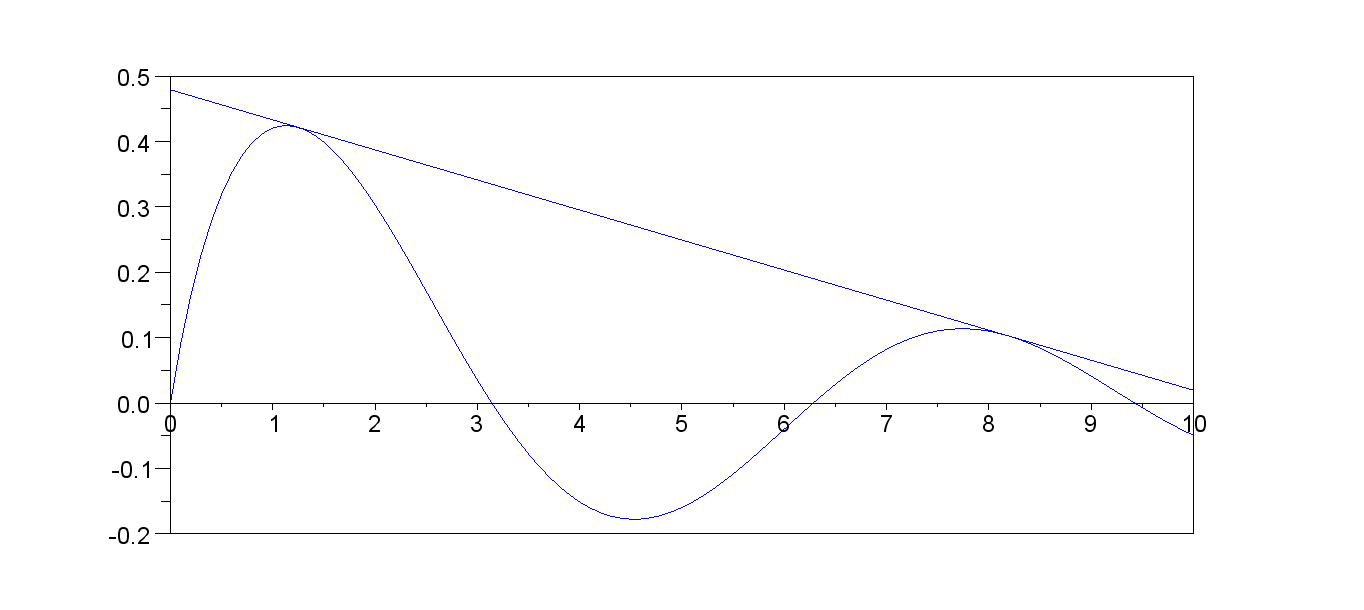
\includegraphics[width=\textwidth]{cap_nlinsis/pics/curva_Q23}
		\caption{Reta bitangente a uma curva.}
		\label{pic:bitang}
	\end{figure}

 \begin{resp}
  $y=mx+b$ com $m\approx - 0.0459710 $ e $b\approx 0.479237$

 Uma metodologia possível para resolver este problema é dada a seguir:

Sejam $x_1$ e $x_2$ as abscissas dos dois pontos em que a reta tangencia a curva. A equação da reta bitangente assume a seguinte forma:
$$y=f(x_1) + m(x-x_1) $$
onde o coeficiente angular $m$ é dado por
$$m=\frac{f(x_2)-f(x_1)}{x_2-x_1}$$

Da condição de tangência, temos que o coeficiente angular da reta, $m$, deve igual à derivada da função $f(x)$ nos dois pontos de tangência.
$$m=f'(x_1)=f'(x_2)$$
E sabemos que:
$$f'(x)=\frac{\cos(x)}{1+x}-\frac{\sin(x)}{(1+x)^2}.$$

Assim, podemos reescrever o problema como
\begin{eqnarray*}
\frac{\cos(x_1)}{1+x_1}-\frac{\sin(x_1)}{(1+x_1)^2}-\frac{\cos(x_2)}{1+x_2}+\frac{\sin(x_2)}{(1+x_2)^2}=0\\
\frac{\cos(x_1)}{1+x_1}-\frac{\sin(x_1)}{(1+x_1)^2}-\frac{f(x_2)-f(x_1)}{x_2-x_1}=0
\end{eqnarray*}
Este é um sistema não linear de duas incógnitas.

Os valores iniciais para o método podem ser obtidos do gráfico buscando valores próximos aos dois primeiros pontos de máximos. Por exemplo: $x_1^{(0)}=1$ e $x_2^{(0)}=8$. Obtemos $x_1\approx 1,2464783$ e $x_2\approx 8,1782997$ e $m$ pode ser obtido através desses valores.


\end{resp}

\begin{figure}
        \centering
	    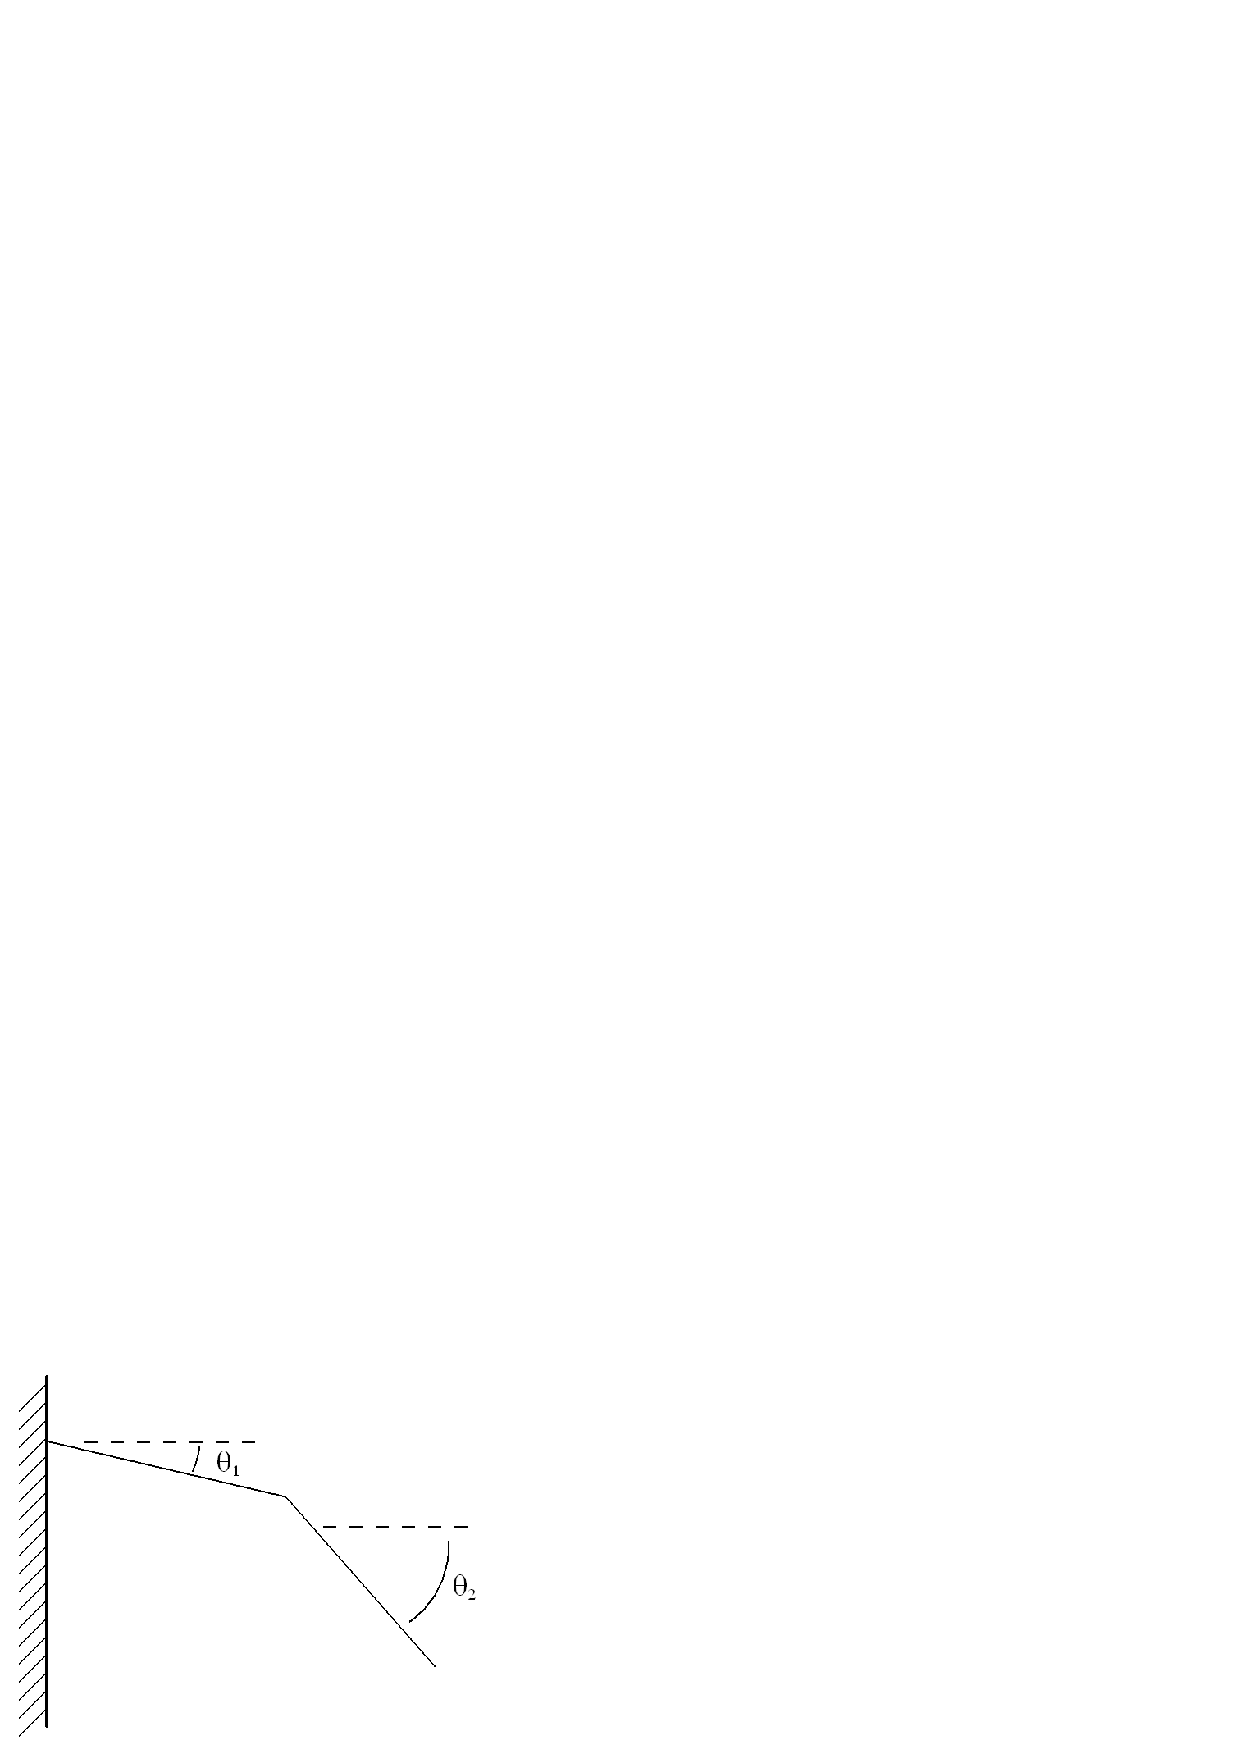
\includegraphics[width=.5\textwidth]{cap_nlinsis/pics/dois_segmentos}
		\caption{Sistema mecânico com dois segmentos.}
		\label{pic:dois_segmentos}
	\end{figure}

\begin{exer}{(Estática)}\label{prob:dois_segmentos} Considere o sistema mecânico constituído de dois segmentos de mesmo comprimento $L$ presos entre si e a uma parede por articulações conforme a Figura~\ref{pic:dois_segmentos}.

O momento em cada articulação é proporcional à deflexão com constante de proporcionalidade $k$. Os segmentos são feitos de material homogêneo de peso $P$. A condição de equilíbrio pode ser expressa em termos dos ângulos $\theta_1$ e $\theta_2$ conforme:
\begin{eqnarray*}
k\theta_1&=& \frac{3PL}{2}\cos\theta_1 + k\left(\theta_2-\theta_1\right)\\
k\left(\theta_2-\theta_1\right)&=& \frac{PL}{2}\cos\theta_2
\end{eqnarray*}
Considere $P=100N$, $L=1m$ e calcule os ângulos $\theta_1$ e $\theta_2$ quando:
\begin{itemize}
\item[a)] $k=1000$ Nm/rad
\item[b)] $k=500$ Nm/rad
\item[c)] $k=100$ Nm/rad
\item[d)] $k=10$ Nm/rad
\end{itemize}
\noindent {\bf Obs:}Você deve escolher valores para iniciar o método. Como você interpretaria fisicamente a solução para produzir palpites iniciais satisfatórios? O que se altera entre o caso a e o caso d?
\end{exer}

\begin{resp}
$\left(0.1956550;0.2441719 \right)$, $\left(0.3694093;0.4590564\right) $, $\left( 0.9990712;1.1865168  \right)$ e $\left(1.4773606;1.5552232 \right)$
\end{resp}


\begin{exer}{(estática - problemas de três variáveis)} Considere, agora, o sistema mecânico semelhante ao do Problema~\ref{prob:dois_segmentos}, porém constituído de três segmentos de mesmo comprimento $L$ presos entre si e a uma parede por articulações.

O momento em cada articulação é proporcional à deflexão com constante de proporcionalidade $k$. Os segmentos são feitos de material homogêneo de peso $P$. A condição de equilíbrio pode ser expressa em termos dos ângulos $\theta_1$, $\theta_2$ e $\theta_3$ conforme:
\begin{eqnarray*}
k\theta_1&=& \frac{5PL}{2}\cos\theta_1 + k\left(\theta_2-\theta_1\right)\\
k\left(\theta_2-\theta_1\right)&=& \frac{3PL}{2}\cos\theta_2+k\left(\theta_3-\theta_2\right)\\
k\left(\theta_3-\theta_2\right)&=& \frac{PL}{2}\cos\theta_3
\end{eqnarray*}
Considere $P=10$N, $L=1$m e calcule os ângulos $\theta_1$, $\theta_2$ e $\theta_3$ quando:
\begin{itemize}
\item[a)] $k=1000$Nm/rad
\item[b)] $k=100$Nm/rad
\item[c)] $k=10$Nm/rad
\end{itemize}
\end{exer}
\begin{resp}
$\left(0.0449310; 0.0648872; 0.0698750  \right)$, $\left(0.3981385; 0.5658310; 0.6069019  \right)$, \\
$\left(1.1862966;1.4348545;1.480127  \right)$
\end{resp}


\begin{figure}
        \centering
	    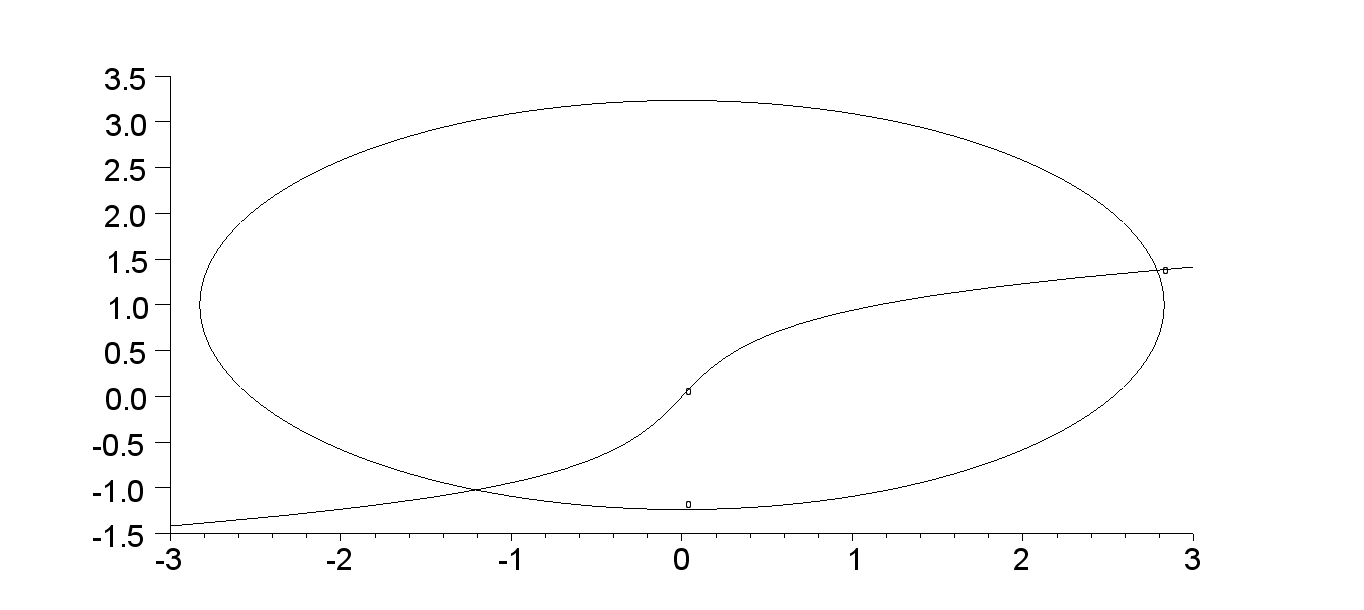
\includegraphics[width=.5\textwidth]{cap_nlinsis/pics/inter_curvas}
		\caption{intersecção entre duas curvas.}
		\label{pic:inter_curvas}
	\end{figure}

\begin{exer}  Considere o problema de encontrar os pontos de intersecção das curvas descritas por (ver Figura~\ref{pic:inter_curvas}):
\begin{eqnarray*}
\frac{x^2}{8}+\frac{(y-1)^2}{5}&=&1\\~\\
\tan^{-1}(x)+x&=&y+y^3
\end{eqnarray*}
 Com base no gráfico, encontre soluções aproximadas para o problema e use-as para iniciar o método de Newton-Raphson. Encontre as raízes com erro inferior a $10^{-5}$.
\end{exer}

\begin{resp}
$\left(-1,2085435, -1,0216674 \right)$ e $\left(2,7871115, 1,3807962\right)$

\ifisscilab
Exemplo de implementação:
\begin{verbatim}
function z=f(x,y)
    z=x^2/8+(y-1)^2/5-1
endfunction
function z=g(x,y)
    z=atan(x)+x-y-y^3
endfunction

contour([-3:.1:3],[-2:.1:4],f,[0 0])
contour([-3:.1:3],[-2:.1:4],g,[0 0])

function y=F(x)
    y(1)=f(x(1),x(2))
    y(2)=g(x(1),x(2))
endfunction
function y=JF(x)
    y(1,1)=x(1)/4
    y(1,2)=2*(x(2)-1)/5
    y(2,1)=1/(1+x(1)^2)+1
    y(2,2)=-1-3*x(2)^2
endfunction

//primeiro ponto
//x=[-1.2;-1.0]

//segundo ponto
//x=[2.8;1.4]

x=x-JF(x)\F(x)   // 4 vezes
\end{verbatim}
\fi
\end{resp}




\begin{exer} Considere o sistema de equações dado por
\begin{eqnarray*}
\frac{(x-3)^2}{16}+\frac{(y-1)^2}{36}&=&1\\
\tanh(x)+x&=&2\sin y-0.01y^3
\end{eqnarray*}
Usando procedimentos analíticos, determine uma região limitada do plano onde se encontram necessariamente todas as raízes do problema.
Encontre as raízes desse sistema com pelo menos quatro dígitos significativos corretos usando o método de Newton. Você deve construir o método de Newton indicando as funções envolvidas e calculando a matriz jacobiana analiticamente. Use que $\frac{d}{du}\tanh u = 1-\tanh^2u$, se precisar.
\end{exer}
\begin{resp}
 A primeira curva trata-se de uma elipse de centro $(3,1)$ e semi-eixos 4 e 6, portanto seus pontos estão contidos no retângulo $-1\leq x \leq 7$ e $-5\leq y \leq 7$.

As soluções são $\left( -0,5384844 , -1,7978634\right)$ e $\left(2,8441544, 6,9954443\right)$.

\ifisscilab
Uma possível implementação é
\begin{verbatim}

function z=f(x,y)
    z=(x-3)^2/16+(y-1)^2/36-1
endfunction

function z=g(x,y)
    z=atan(x)+x-sin(y)-0.01*y^3
endfunction

contour([-1:.1:7],[-5:.1:7],f,[0 0])
contour([-1:.1:7],[-5:.1:7],g,[0 0])

function y=F(x)
    y(1)=f(x(1),x(2))
    y(2)=g(x(1),x(2))
endfunction
function y=JF(x)
    y(1,1)=(x(1)-3)/8
    y(1,2)=(x(2)-1)/18
    y(2,1)=1/(1+x(1)^2)+1
    y(2,2)=-cos(x(2))-0.03*x(2)^2
endfunction
 \end{resp}

//primeiro ponto
//x=[-.5;-2.0]

//segundo ponto
//x=[3;7]

x=x-JF(x)\F(x)   // 4 vezes
\end{verbatim}
\fi
\end{resp}



\begin{exer}(Otimização)\label{nlinsis:usinas} Uma indústria consome energia elétrica de três usinas fornecedoras. O custo de fornecimento em reais por hora como função da potência consumida em kW é dada pelas seguintes funções
\begin{eqnarray*}
C_1(x)&=&10+.3x+10^{-4}x^2+3.4\cdot 10^{-9}x^4\\
C_2(x)&=&50+.25x+2\cdot 10^{-4}x^2+4.3\cdot 10^{-7}x^3\\
C_3(x)&=&500+.19x+5\cdot 10^{-4}x^2+1.1\cdot 10^{-7}x^4
\end{eqnarray*}
Calcule a distribuição de consumo que produz custo mínimo quando a potência total consumida é $1500kW$. Dica: Denote por $x_1$, $x_2$ e $x_3$ as potências consumidas das usinas 1, 2 e 3, respectivamente.  O custo total será dado por $C(x_1,x_2,x_3)=C_1(x_1)+C_2(x_2)+C_3(x_3)$ enquanto o consumo total é $x_1+x_2+x_3=1500$. Isto é, queremos minimizar a função custo total dada por:
$$C(x_1,x_2,x_3)=C_1(x_1)+C_2(x_2)+C_3(x_3)$$
restrita à condição
$$G(x_1,x_2,x_3)=x_1+x_2+x_3-1500=0.$$
Pelos multiplicadores de Lagrange, temos que resolver o sistema dado por:
\begin{eqnarray*}
\nabla C(x_1,x_2,x_3) &=& \lambda \nabla G(x_1,x_2,x_3)\\
G(x_1,x_2,x_3)&=&0
\end{eqnarray*}
\end{exer}

\begin{resp}
 $(x_1,x_2,x_3)\approx (453,62,~ 901,94,~ 144,43)$
\end{resp}


\begin{exer} \label{nlinsis:prob_ajuste_eax} Encontre a função do tipo $f(x)=Ab^{x}$ que melhor aproxima os pontos $(0,~3,1)$, $(1,~4,4)$ e $(2,~6,7)$ pelo critério dos mínimos quadrados. Dica: Você deve encontrar os valores de $A$ e $b$ que minimizam o resíduo dado por
$$R=\left[3,1-f(0)\right]^2+\left[4,4-f(1)\right]^2+\left[6,7-f(2)\right]^2.$$
{\bf Dica:} Para construir aproximações para resposta e iniciar o método, considere a função $f(x)=Ab^x$ que passa pelo primeiro e terceiro ponto.
\end{exer}
\begin{resp}
Inicialização do método: $A^{(0)}= 3,1$ e $b^{(0)}= \sqrt{\frac{6,7}{3,1}}$
$A\approx  3.0297384 $ e $b\approx 1.4835346$.
\end{resp}




 \begin{exer}Encontre o valor máximo da função $$f(x,y)=-x^4-y^6+3xy^3-x$$ na região $(x,y)\in [-2,0]\times [-2,0]$
 seguindo os seguintes passos:
\begin{itemize}
  \item[a)] Defina a função $z=f(x,y)=-x^4-y^6+3xy^3-x$ e trace o gráfico de contorno na região.
  \item[b)] Com base no gráfico, encontre valores aproximados para as coordenadas $xy$ do ponto de máximo.
  \item[c)] Sabendo que o ponto de máximo acontece quando o gradiente é nulo, escreva o problema como um sistema de duas equações não lineares e duas incógnitas.
  \item[d)] Implemente o método de Newton.
\end{itemize}
\end{exer}
 \begin{resp}
 $f(-1,1579702, -1,2020694)\approx 2.376985$

\ifisscilab
Um exemplo de implementação no Scilab é:
\begin{verbatim}
deff('z=f(x,y)','z=-x^4-y^6+3*x*y^3-x')
contour([-2:.01:0],[-2:.01:0],f,[ 0:.2: 3])
deff('z=F(x)','z=[-4*x(1)^3+3*x(2)^3-1;-6*x(2)^5+9*x(1)*x(2)^2]')
deff('z=JF(x)','z=[-12*x(1)^2,9*x(2)^2;9*x(2)^2,-30*x(2)^4+18*x(1)*x(2)]')
x=[-1.2;-1.2]
x=x-JF(x)\F(x)
x=x-JF(x)\F(x)
x=x-JF(x)\F(x)
x=x-JF(x)\F(x)
mprintf('f(%f,%f)=%f',x(1),x(2),f(x(1),x(2)))
\end{verbatim}
\fi
\end{resp}



 \begin{exer}A função $f(x,y,z)=\sin(x)+\sin(2y)+\sin(3z)$ possui um máximo quando $x=\pi/2$, $y=\pi/4$ e $z=\pi/6$. Calcule numericamente este ponto.
 \end{exer}


 \begin{exer}\label{prob_sis3} Encontre as raizes do problema
 \begin{eqnarray*}
 3x-\cos(yz+z)-1/2&=&0\\
 4x^2-25y^2+0.4y+2&=&0\\
 e^{-xy}+2x-5z&=&10
 \end{eqnarray*}
 no cubo $|x|<2, |y|<2, |z|<2.$
 Dica: Reduza a um problema de duas incógnitas e use recursos gráficos para aproximar as raízes na região.
 \end{exer}

 \begin{resp}
 $x\approx 0,2982646, y\approx -0,2990796, z\approx- 1,6620333$  e $x\approx -0,0691328, y\approx 0,2923039, z\approx -0,8235705$.
 \end{resp}


\begin{exer}  Considere o seguinte sistema de equações não lineares:
\begin{eqnarray}
x_1-x_2&=&0\nonumber\\
-x_{j-1}+5(x_j+x_j^3)-x_{j+1}&=&10\exp(-j/3),~~ 2\leq j \leq 10\nonumber\\
x_{11}&=&1
\end{eqnarray}
\begin{itemize}
\item [a)] Escreva este sistema na forma $F(x)=0$ onde $x=\left[\begin{array}{c} x_1\\ x_2\\ \vdots \\ x_{11}\end{array}\right]$ e calcule analiticamente a matriz jacobiana $\frac{\partial (F_1,\ldots, F_{11})}{\partial (x_1,\ldots x_{11})}$. Dica: Use a regularidade nas expressões para abreviar a notação.
\item [b)] Construa a iteração para encontrar a única solução deste problema pelo método de Newton e, usando esse método, encontre uma solução aproximada com erro absoluto inferior a $10^{-4}$.
\end{itemize}
\end{exer}

\begin{resp}
$$F\left(x\right)=\left[
\begin{array}{c}
x_1-x_2\\[.2cm]
-x_{1}+5(x_2+x_2^3)-x_{3}-10\exp(-2/3)\\[.2cm]
-x_{2}+5(x_3+x_3^3)-x_{4}-10\exp(-3/3)\\[.2cm]
-x_{3}+5(x_4+x_4^3)-x_{5}-10\exp(-4/3)\\[.2cm]
\vdots\\
-x_{9}+5(x_{10}+x_{10}^3)-x_{11}-10\exp(-10/3)\\[.2cm]
x_{11}-1
\end{array}\right] $$

$$J_F(x)=\left[
\begin{array}{ccccccc}
1& -1 &0 &0 &0&\ldots & 0\\[.2cm]
-1&5(1+3x_2^2)& -1&0&0&\ldots & 0\\[.2cm]
0&-1&5(1+3x_3^2)& -1&0&\ldots & 0\\[.2cm]
0&0&-1&5(1+3x_4^2)& -1&\ldots & 0\\[.2cm]
\vdots &\vdots &\vdots &\vdots &&\ddots&\vdots\\[.2cm]
0&0&0&0&0&\cdots&1
\end{array}
\right]
$$

\ifisscilab
Exemplo de implementação no Scilab:
\begin{verbatim}
function y=F(x)
    y(1)=x(1)-x(2)
    for j=2:10
        y(j)=-x(j-1)+5*(x(j)+x(j)^3)-x(j+1)-10*exp(-j/3)
    end
    y(11)=x(11)-1
endfunction

function y=JF(x)
    y=zeros(11,11)

    y(1,1)=1
    y(1,2)=-1
    for j=2:10

        y(j,j-1)=-1
        y(j,j)=5*(1+3*x(j)^2)
        y(j,j+1)=-1
    end
    y(11,11)=1
endfunction
\end{verbatim}
\fi

Resposta final: 0,80447, 0,80447, 0,68686, 0,57124, 0,46535,
0,37061, 0,28883, 0,22433, 0,19443, 0,28667,  1
\end{resp}


\begin{exer} Considere a função
$$f(x,y)=\frac{e^{-(x-1)^2-(y-2)^2}}{1+x^2+y^2}$$
\begin{itemize}
\item[a)] Encontre o valor máximo desta função.
\item[b)] Usando multiplicadores de Lagrange, encontre o valor máximo desta função restrito à condição $$(x-1)^2+(y-2)^2=1.$$
\item[c)] Parametrize a circunferência para transformar o problema de máximo com restrição em um problema de uma única variável. Resolva usando as técnicas de equações lineares de uma variável.
\end{itemize}

\end{exer}
\begin{resp}
$f(0,8108792, 1,6217584)\approx 0,1950369$ e $f(0,5527864, 1,1055728 )\approx 0,1455298 $
\end{resp}



\section{Linearização de uma função de várias variáveis}
Nesta seção, discutimos de forma distinta e mais rigorosa os conceitos de matriz jacobiana e linearização de uma função de várias variáveis.\index{matriz!jacobiana}
\subsection{Gradiente}

Considere primeiramente uma função $f:\mathbb{R}^n\to \mathbb{R}$, ou seja, uma função que mapeia n variáveis reais em um único real, por exemplo:
$$f(x)=x_1^2+x_2^2/4$$

Para construirmos a linearização, fixemos uma direção no espaço $\mathbb{R}^n$, ou seja, um vetor $v$:
$$v=[v_1,  v_2,  \cdots,  v_n]^T$$

Queremos estudar como a função $f(x)$ varia quando ``andamos'' na direção $v$ a partir do ponto $x^{(0)}$. Para tal, inserimos um parâmetro  real pequeno $h$, dizemos que $$x=x^{(0)}+hv$$ e definimos a função auxiliar
$$g(h)=f(x^{0}+hv).$$
Observamos que a função $g(h)$ é uma função de $\mathbb{R}$ em $\mathbb{R}$.

A linearização de $g(h)$ em torno de $h=0$ é dada por

$$g(h)=g(0) + hg'(0) +O(h^2)$$
Observamos que $g(h)=f(x^{(0)}+hv)$ e $g(0)=f(x^{(0)})$. Precisamos calcular $g'(0)$:

\begin{eqnarray*}
g'(h)=\frac{d}{dh}g(h)=\frac{d}{dh}f(x^{(0)}+hv).
\end{eqnarray*}
Pela regra da cadeia temos:
\begin{eqnarray*}
\frac{d}{dh}f(x^{(0)}+hv)= \sum_{j=1}^n \frac{\partial f}{\partial x_j}\frac{d x_j}{d h}.
\end{eqnarray*}

Observamos que $x_j=x^{(0)}_j+hv_j$, portanto
$$\frac{d x_j}{d h}=v_j$$
Assim:
\begin{eqnarray*}
\frac{d}{dh}f(x^{(0)}+hv)= \sum_{j=1}^n \frac{\partial f}{\partial x_j}v_j.
\end{eqnarray*}
Observamos que esta expressão pode ser vista como o produto interno entre o gradiente de $f$ e o vetor $v$:
\begin{eqnarray*}
\nabla f = \left[
\begin{matrix}
\frac{\partial f}{\partial x_1} \\
\frac{\partial f}{\partial x_2} \\
\vdots\\
\frac{\partial f}{\partial x_n}
\end{matrix}
\right] \qquad v=\left[
\begin{matrix}
v_1\\
v_2\\
\vdots\\
v_n
\end{matrix}
\right]
\end{eqnarray*}

Na notação cálculo vetorial escrevemos este produto interno como $\nabla f \cdot v = v \cdot \nabla f$ na notação de produto matricial, escrevemos $\left(\nabla f\right)^T v = v^T\nabla f$. Esta quantidade é conhecida como {\bf derivada direcional} de $f$ no ponto $x^{(0)}$ na direção $v$, sobretudo quando $\|v\|=1$.


Podemos escrever a linearização
$g(h)=g(0) + hg'(0) +O(h^2)$ como
$$f(x^{(0)}+hv)=f(x^{(0)})+ h \nabla^T\! f(x^{(0)})\!~v  + O(h^2)$$

Finalmente, escrevemos $x=x^{(0)}+hv$, ou seja, $hv=x-x^{(0)}$
$$f(x)=f(x^{(0)})+ \nabla^T\! f(x^{(0)})\!~(x-x^{(0)})   + O(\|x-x^{(0)}\|^2)$$

\begin{obs} Observe a semelhança com a linearização no caso em uma dimensão. A notação $\nabla^T\! f(x^{(0)})$ é o transposto do vetor gradiente associado à função $f(x)$ no ponto $x^{(0)}$:
$$\nabla^T f(x^{(0)})=\left[\frac{\partial f\left(x^{(0)}\right)}{\partial x_1},~~ \frac{\partial f\left(x^{(0)}\right)}{\partial x_2},~~ \cdots,~\frac{\partial f\left(x^{(0)}\right)}{\partial x_n}\right]$$
\end{obs}

\subsection{Matriz jacobiana}\index{matriz!jacobiana}
Interessamo-nos, agora, pela linearização da função $F:\mathbb{R}^n\to \mathbb{R}^n$. Lembramos que $F(x)$ pode ser escrita como um vetor de funções $f_j:\mathbb{R^n}\to\mathbb{R}$:
\begin{equation*}
  F(x)=\left[\begin{matrix}
      f_1(x)\\
      f_2(x)\\
      \vdots\\
      f_n(x)
    \end{matrix}\right]
\end{equation*}
Linearizando cada uma das funções $f_j$, temos:
\begin{eqnarray*}
F(x)&=&\underbrace{\left[
\begin{array}{c}
f_1\left(x^{(0)}\right)+\nabla^T\! f_1(x^{(0)})\!~\left(x-x^{(0)}\right)   + O(\|x-x^{(0)}\|^2)\\~\\
f_2\left(x^{(0)}\right)+\nabla^T\! f_2(x^{(0)})\!~\left(x-x^{(0)}\right)   + O(\|x-x^{(0)}\|^2)\\~\\
\vdots\\~\\
f_n\left(x^{(0)}\right)+\nabla^T\! f_n(x^{(0)})\!~\left(x-x^{(0)}\right)   + O(\|x-x^{(0)}\|^2)
\end{array}
\right]}_{\text{Vetor coluna}}
\end{eqnarray*}
ou, equivalentemente:
\begin{eqnarray*}
 F(x) &=&\underbrace{\left[
\begin{array}{c}
f_1\left(x^{(0)}\right)\\~\\
f_2\left(x^{(0)}\right)\\~\\
\vdots\\~\\
f_n\left(x^{(0)}\right)
\end{array}
\right]}_{\text{Vetor coluna}}+
\underbrace{\left[
\begin{array}{c}\nabla^T\! f_1(x^{(0)})\\~~\\
\nabla^T\! f_2(x^{(0)})\\~~\\
\vdots\\~~\\
\nabla^T\! f_n(x^{(0)})
\end{array}
\right]}_{\text{Matriz jacobiana}}\underbrace{\left(x-x^{(0)}\right)}_{\text{Vetor coluna}}+O(\|x-x^{(0)}\|^2)
\end{eqnarray*}

Podemos escrever a linearização de $F(x)$ na seguinte forma mais enxuta:
$$F(x)=F\left(x^{(0)}\right)+ J_F(x^{(0)})\left(x-x^{(0)}\right) + O\left(\left\|x-x^{(0)}\right\|^2\right) $$

A matriz jacobiana $J_F$ é matriz cujas linhas são os gradientes transpostos de $f_j$, ou seja:
$$J_F= \frac{\partial(f_1,f_2,\ldots,f_n)}{\partial(x_1,x_2,\ldots,x_n)}=\left[
\begin{array}{ccccc}
\frac{\partial f_1}{\partial x_1}&\frac{\partial f_1}{\partial x_2}&\cdots&\frac{\partial f_1}{\partial x_n}\\~\\
\frac{\partial f_2}{\partial x_1}&\frac{\partial f_2}{\partial x_2}&\cdots&\frac{\partial f_2}{\partial x_n}\\~\\
\vdots&\vdots&\ddots&\vdots\\~\\
\frac{\partial f_n}{\partial x_1}&\frac{\partial f_n}{\partial x_2}&\cdots&\frac{\partial f_n}{\partial x_n}\\~\\
\end{array}
\right]
$$
A matriz jacobiana de uma função ou simplesmente, o jacobiano de uma função $F(x)$ é a matriz formada pelas suas derivadas parciais:
$$\left(J_F\right)_{ij}=\frac{\partial f_i}{\partial x_j}$$


\begin{ex} Calcule a matriz jacobiana da função
$$F(x)=\left[
\begin{array}{c}
\frac{x_1^2}{3}+x_2^2-1\\~\\
x_1^2+\frac{x_2^2}{4}-1
\end{array}
\right]$$

$$J_F=\left[
\begin{array}{cc}
\frac{\partial f_1}{\partial x_1} & \frac{\partial f_1}{\partial x_2}\\~\\
\frac{\partial f_2}{\partial x_1} & \frac{\partial f_2}{\partial x_2}\\
\end{array}
\right]=\left[
\begin{array}{cc}
\frac{2x_1}{3} & 2x_2\\~\\
2x_1&\frac{x_2}{2}
\end{array}
\right]
$$
\end{ex}

%\end{document}
